\setchapterpreamble[u]{\margintoc}
\chapter{Summary and Outlook}
\labch{summary}

The aim of this thesis was to measure the flavor composition of astrophysical neutrinos using the High Energy Starting Event (HESE) sample, collected over approximately 12 years. This analysis involved classifying HESE events into three morphological categories: single cascades, tracks, and double cascades. Each morphology typically correlates with a unique neutrino flavor interaction, so this classifier, known as a particle identifier or ternary classifier, is useful for distinguishing neutrino types. Appropriate variables were selected to build Monte Carlo probability density functions (PDFs) that effectively differentiate signal from background events. For electron and muon neutrinos ($\nu_e$ and $\nu_\mu$), single cascades and tracks were analyzed against atmospheric neutrino backgrounds, whereas tau neutrino ($\nu_\tau$) backgrounds predominantly originated from other flavor misclassifications. A likelihood fit was then applied to events with reconstructed energies above 60 TeV.

In the double cascade topology, events arising from $\nu_\tau$ charged-current (CC) interactions exhibit a relationship between the reconstructed total energy deposited and the length of the reconstructed double cascade. This feature is absent in misclassified neutral-current, $\nu_e$-CC, and $\nu_\mu$-CC events. This unique topology, resolvable at high energies, helps break the $\nu_e$-$\nu_\tau$ degeneracy at energies above $\sim 100$ TeV, thereby improving direct sensitivity to each flavor in combination with single-cascade and track topologies. The work in this thesis focused on three main parts: updating the ternary classifier with recent ice models, reconstruction tables, and simulations; performing a likelihood fit to measure the flavor composition using an additional four years of HESE data compared to prior studies; and producing Monte Carlo simulations targeted at the future IceCube-Gen2 detector to extend the classifier to the next-generation detector.

The classifier update was comprehensive, entailing adjustments to the neutrino weight in the sample, which influences expected event rates and Monte Carlo PDFs for reconstructed quantities. This included a new classification to reduce background events from high-energy $\nu_e$ single cascades near the Glashow resonance, alongside corrections for assumed neutrino interaction cross-sections in Glashow events. Adjustments to the CC tau neutrino events were also made to account for the polarized states of tau leptons, affecting the energy distribution of decay products, an important variable in double-cascade reconstruction. Though no significant differences were observed at the analysis level, these corrections were retained.

Further, updates incorporated a refined ice model, SPICE-Bfr, for reconstruction. Because the reconstruction method relies on tabulated light yield—generated with a specific ice model—and the double-cascade length reconstruction is particularly sensitive to ice anisotropies, the new model was used as it aligns best with current data. Additionally, a novel simulation technique called the SnowStorm technique was applied, where detector systematics varied continuously rather than requiring discrete Monte Carlo sets.

In performing the likelihood fit, parameters and flux components were updated from prior iterations. For uncertainties in detector systematics, the Snowstorm approach was used, where detector parameters vary continuously to capture systematic uncertainties. While many other parameters affecting cosmic-ray spectrum features were included, they had limited impact on the fit. A key addition was the inelasticity parameter, which influences the energy deposition and thereby normalizes the observed spectra. Updated software was also employed in this analysis.

In applying the first two steps of the updated methodology, the 7.5-year dataset saw an unexpected surplus of double-cascade events compared to previous data unblindings. Investigation revealed this excess was likely due to incorporating the high-quantum-efficiency DeepCore DOMs in the reconstruction, which hadn’t been done previously. However, the simulation predictions did not match the observed data. A deeper investogation discovered a bug in the charge template used in data calibration files. The data files used older template while simulation had been updated with the new ones. This inconsistency between simulation and data was problematic for maximum-likelihood energy estimation methods that rely on charge templates. Ultimately, DeepCore DOMs were removed from the reconstruction, and the likelihood fit was re-performed, leading to a final 12-year dataset with 5 double cascades, 64 single cascades, and 28 track events above 60 TeV. The resulting best-fit flavor composition was $\nu_e : \nu_\mu : \nu_\tau=0.19:0.43:0.38$, consistent with previous measurements, indicating a preference for a muon-damped source scenario but insufficient sensitivity to reject alternative models such as the no-astrophysical $\nu_\tau$ hypothesis at even a $1\sigma$ level, though designed for $2\sigma$ sensitivity. Monte Carlo pseudo-experiments demonstrated that many observed events fall in bins where the signal-to-background ratio is low, hampering the fit’s ability to distinguish signal from background effectively.

The analysis in this thesis underscores the challenges posed by limited statistics in the HESE sample for flavor composition measurements. The low number of double-cascade events constrains the statistical power, which could be significantly improved by including additional high-statistics samples, particularly cascades and tracks, to better constrain $\nu_e$ and $\nu_\mu$ fractions. The findings suggest that the classifier and the analysis method could benefit from revisions before future fits, given the sensitivity of the double-cascade reconstruction to minor methodological changes. For instance, while double-cascade events like \textbf{Double Double} remain consistently classified in every configurations (and even analyses, including the one presented here and both \sidecite{Juliana_paper,CNN_tau} ), the inclusion or exclusion of DeepCore DOMs and slight changes in ice models cause notable classification shifts, questioning the classifier's robustness. The cut values used to separate signal from background were initially derived assuming a harder neutrino flux spectrum, where more high-energy events would increase $\nu_\tau$ counts \sidecite{marcel_thesis}. Since the HESE spectrum is softer, these cut values should be re-evaluated to enhance sample purity. The simulations were generated with an older ice model version, which further impacts data-mc agreement and could improve the results if updated. Although the analysis did not yield a groundbreaking measurement, it illuminated critical issues with the reconstruction methods, suggesting areas for improvement in future studies. 

\begin{figure}[h]
    
    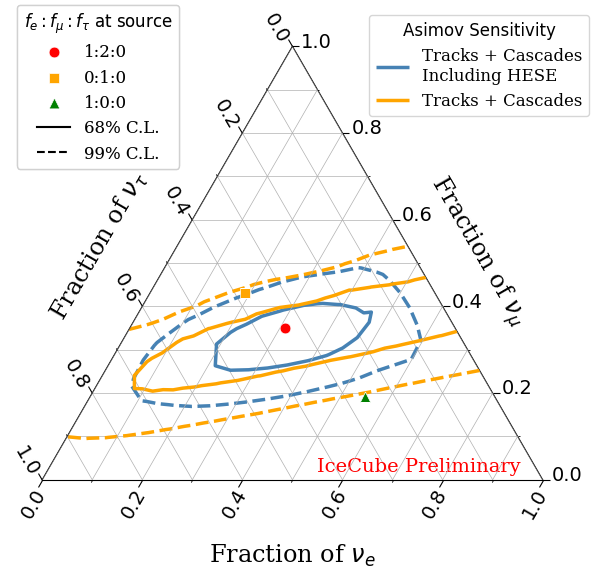
\includegraphics{./figures/results/3D_Combined.png}


    \caption{The sensitivity to measure flavor composition by combining 12 years of HESE sample with current GlobalFit sample \cite{globalfit_icrc}, for an astrophysical neutrino spectrum following the single unbroken power-law given as $E^{-2.3}$, with a flavor composition of $\nu_e : \nu_\mu : \nu_\tau = 1 : 1 : 1$.
    }
    \labfig{globalfit}
\end{figure}

A combined global fit using multiple samples could offer stronger constraints on flavor ratios in future analyses. As shown in \reffig{globalfit} in projected sensitivity, adding 12 years of HESE data to a recently unblinded global fit\sidenote{Note that the figure is produced assuming a single power law of index 2.3, and not the broken power law result of the globalfit \cite{globalfit_icrc}} could provide around $3\sigma$ sensitivity to rule out models like the neutron-beam scenario, assuming an equitable flavor partition. Additionally, exploring alternative detection techniques, such as convolutional neural networks (CNNs) for double-pulse signature recognition, could aid in $\nu_\tau$ detection, especially for lower-energy events. This double-pulse technique—analogous to double-cascade identification—could expand analysis to events up to a few hundred TeV, where pulses on DOMs are sufficiently close to register as two distinct signals. This method is already used within IceCube \cite{CNN_tau}, providing a foundation for future $\nu_\tau$ detection efforts.

As highlighted, precise knowledge of the ice model is essential for reconstruction accuracy. IceCube's Upgrade project will place new calibration devices with improved resolution to map Antarctic ice properties, enhancing the accuracy of double-cascade length resolution and advancing oscillation studies across a wide energy range \sidecite{AYA}. Future improvements in ice optical property data from these upgrades will support higher fidelity in simulations and more consistent agreement with observed data, which is vital for tau neutrino detection. The larger-scale IceCube-Gen2 project will open even greater possibilities with its 8-fold volume increase and improved PMT modules, expanding sensitivity for astrophysical neutrino detection across broader energy scales.  IceCube-Gen2 will also support more accurate cascade angular reconstruction, which will aid in $\nu_\tau$ identification and benefit follow-up observations with electromagnetic telescopes due to the relatively low atmospheric background in $\nu_\tau$ signals. This expanded scope could even facilitate identification of changes in neutrino production scenarios at different energy levels, potentially revealing dominant source classes at specific energy thresholds. By combining optical and radio arrays, Gen2 could reach energies accessible to cosmogenic neutrinos, which are otherwise limited by the GZK cutoff in cosmic-ray studies. The new optical sensors and improved angular resolution in double-cascade detection will not only enhance $\nu_\tau$ identification but may also offer a nearly background-free signal, providing invaluable data for locating and studying astrophysical neutrino sources.


